% ------------------------------------------------------------------------------
% TYPO3 CMS 7.2 - What's New - Chapter "Introduction" (English Version)
%
% @author	Michael Schams <schams.net>
% @license	Creative Commons BY-NC-SA 3.0
% @link		http://typo3.org/download/release-notes/whats-new/
% @language	English
% ------------------------------------------------------------------------------
% LTXE-CHAPTER-UID:		16517900-07a67f43-fe9f3e35-7e924788
% LTXE-CHAPTER-NAME:	Introduction
% ------------------------------------------------------------------------------

\section{Введение}
\begin{frame}[fragile]
	\frametitle{Введение}

	\begin{center}\huge{Введение}\end{center}
	\begin{center}\huge{\color{typo3darkgrey}\textbf{Факты}}\end{center}

\end{frame}

% ------------------------------------------------------------------------------
% LTXE-SLIDE-START
% LTXE-SLIDE-UID:		ef15b6b4-9c85ffbf-b4d95c31-6e03498a
% LTXE-SLIDE-ORIGIN:	6d5e9f3e-f9d9677e-43d7d497-e80ba9ef English
% LTXE-SLIDE-TITLE:		TYPO3 CMS 7.2 - The Facts
% ------------------------------------------------------------------------------
\begin{frame}[fragile]
	\frametitle{Введение}
	\framesubtitle{TYPO3 CMS 7.2 - факты}

	\begin{itemize}
		\item Дата выхода: 28 April 2015
		\item Тип: "Sprint Release"
		\item Видение: охват, инновации, доступность
		\item Фокус: Внешний интерфейс / Frontend
	\end{itemize}

	\begin{figure}
		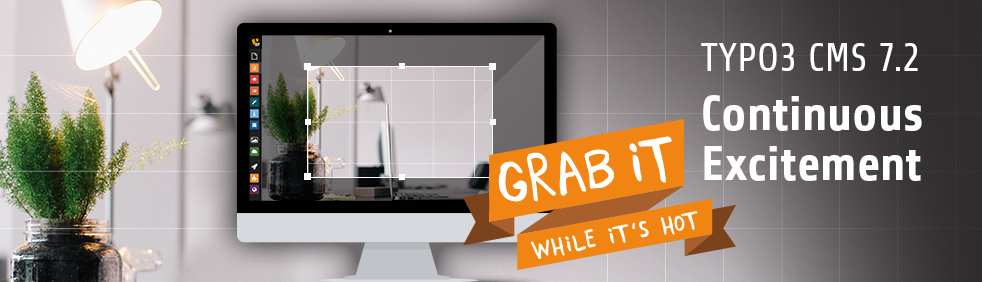
\includegraphics[width=0.95\linewidth]{Introduction/typo3cms72-teaser.png}
	\end{figure}

\end{frame}

% ------------------------------------------------------------------------------
% LTXE-SLIDE-START
% LTXE-SLIDE-UID:		98fcecf5-a359b1bc-1468fa1f-3d64360b
% LTXE-SLIDE-ORIGIN:	759c3860-d5061f6e-2bb0009f-6ea130c8 English
% LTXE-SLIDE-TITLE:		System Requirements
% ------------------------------------------------------------------------------
\begin{frame}[fragile]
	\frametitle{Введение}
	\framesubtitle{Системные требования}

	\begin{itemize}
		\item PHP*:\tabto{4cm}5.5.0 - 5.6.x
		\item MySQL:\tabto{4cm}5.5.x - 5.6.x (no strict mode)
			\item Дисковое пространство:\tabto{4cm}200 МБ мин.
		\item PHP настройки:

			\begin{itemize}
				\item memory\_limit >= 128M
				\item max\_execution\_time >= 240s
					\item compilation option \texttt{--disable-ipv6} \underline{не} должно использоваться
			\end{itemize}

		\item Внутренний интерфейс требует IE >= 9 или любой другой современный браузер

	\end{itemize}

	\vspace{1cm}
	*) Подробности: \href{http://typo3.org/news/article/php-minimum-requirements-for-typo3-cms-7/}{PHP Minimum Requirements for TYPO3 CMS 7}

\end{frame}

% ------------------------------------------------------------------------------
% LTXE-SLIDE-START
% LTXE-SLIDE-UID:		f837c3ea-665571fd-e18603f5-6e515af1
% LTXE-SLIDE-ORIGIN:	70c77c41-e2b83d82-2f182996-98061070 English
% LTXE-SLIDE-TITLE:		Development And Release Timeline
% ------------------------------------------------------------------------------
\begin{frame}[fragile]
	\frametitle{Введение}
	\framesubtitle{График разработки и выхода}

	\begin{figure}
		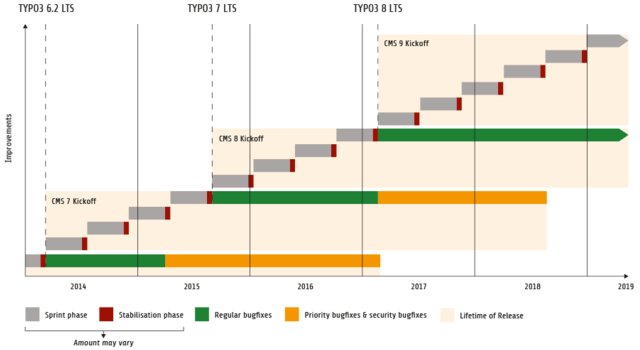
\includegraphics[width=0.90\linewidth]{Introduction/ReleaseAgenda.png}
	\end{figure}

\end{frame}

% ------------------------------------------------------------------------------
% LTXE-SLIDE-START
% LTXE-SLIDE-UID:		ed9366ec-6ed868fc-11d63501-b21132dd
% LTXE-SLIDE-ORIGIN:	b55d3fe9-76807061-d97f3fee-7db1f190 English
% LTXE-SLIDE-TITLE:		TYPO3 CMS Roadmap
% ------------------------------------------------------------------------------
\begin{frame}[fragile]
	\frametitle{Введение}
	\framesubtitle{TYPO3 CMS дорожная карта}

	Примерные даты выхода и их основной фокус:

	\begin{itemize}
			\item v7.0 \tabto{1.0cm}02/дек/2014\tabto{3.4cm}Переработка внутреннего интерфейса часть 1
		\item v7.1 \tabto{1.0cm}24/фев/2015\tabto{3.4cm}Чистка ядра и оптимизация

		\item
			\begingroup
				\color{typo3orange}
					v7.2 \tabto{1.0cm}28/апр/2015\tabto{3.4cm}Внешний интерфейс
			\endgroup

		\item v7.3 \tabto{1.0cm}09/июнь/2015\tabto{3.4cm}Экосистема пакетов, Composer\newline
			\tabto{3.4cm}и работа с расширениями
		\item v7.4 \tabto{1.0cm}04/авг/2015\tabto{3.4cm}Backend Overhaul Vol 2
		\item v7.5 \tabto{1.0cm}29/сен/2015\tabto{3.4cm}\textit{(будет определено...)}
		\item v7.6 \tabto{1.0cm}xx/xxx/2015\tabto{3.4cm}\textbf{TYPO3 CMS 7 LTS} (Long Term Release)
	\end{itemize}

	\smaller
		\url{https://typo3.org/typo3-cms/roadmap/}\newline
		\url{http://typo3.org/news/article/embrace-and-innovate-typo3-cms-7/}
	\normalsize

\end{frame}

% ------------------------------------------------------------------------------
% LTXE-SLIDE-START
% LTXE-SLIDE-UID:		393c8720-7877ac47-664d21e0-e80225ea
% LTXE-SLIDE-ORIGIN:	b0c28f26-c3ca2e99-195954a8-ed76f9d4 English
% LTXE-SLIDE-TITLE:		Installation
% ------------------------------------------------------------------------------
\begin{frame}[fragile]
	\frametitle{Введение}
	\framesubtitle{Установка}

	\begin{itemize}
		\item Официальная процедура установки под Linux/Mac OS X\newline
			(DocumentRoot, например, \texttt{/var/www/site/htdocs}):
		\begin{lstlisting}
			$ cd /var/www/site
			$ wget --content-disposition get.typo3.org/7.2
			$ tar xzf typo3_src-7.2.0.tar.gz
			$ cd htdocs
			$ ln -s ../typo3_src-7.2.0 typo3_src
			$ ln -s typo3_src/index.php
			$ ln -s typo3_src/typo3
			$ touch FIRST_INSTALL
		\end{lstlisting}

		\item Symbolic links под Microsoft Windows:

			\begin{itemize}
				\item Используйте \texttt{junction} под Windows XP/2000
				\item Используйте \texttt{mlink} под Windows Vista и Windows 7
			\end{itemize}

	\end{itemize}
\end{frame}

% ------------------------------------------------------------------------------
% LTXE-SLIDE-START
% LTXE-SLIDE-UID:		a08f9fb6-02c5f1aa-5c6bd0b5-3eef7553
% LTXE-SLIDE-ORIGIN:	48136734-ae508d23-bce5811d-667f8908 English
% LTXE-SLIDE-TITLE:		Upgrade to TYPO3 CMS 7
% ------------------------------------------------------------------------------
\begin{frame}[fragile]
	\frametitle{Введение}
	\framesubtitle{Обновление до TYPO3 CMS 7.x}

	\begin{itemize}
		\item Обновление возможно лишь с TYPO3 CMS 6.2 LTS
		\item TYPO3 CMS < 6.2 должны быть обновлены сначала до TYPO3 CMS 6.2 LTS
		\item Инструкции по обновлению:\newline
			\smaller\url{http://wiki.typo3.org/Upgrade#Upgrading_to_7.2}\normalsize
		\item Официальное руководство TYPO3 "TYPO3 Installation and Upgrading":
			\smaller\url{http://docs.typo3.org/typo3cms/InstallationGuide}\normalsize
		\item Общий подход:
			\begin{itemize}
				\item \smaller Проверка минимальных системных требований \small(PHP, MySQL, etc.) \normalsize
				\item \smaller Просмотр \textbf{deprecation\_*.log} в старой версии TYPO3 \normalsize
				\item \smaller Обновление всех расширений до последней версии \normalsize
				\item \smaller Загрузка новых исходных файлов и запуск Install Tool \textrightarrow Upgrade Wizard \normalsize
				\item \smaller Запуск модуля обзора для внутренних пользователей (опционально) \normalsize
			\end{itemize}
	\end{itemize}

\end{frame}

% ------------------------------------------------------------------------------
